\begin{question}
  \hspace*{\fill} [Note Maximale: 7]\par
  \medskip
  \noindent On considère $f(x) = 2 - x^2$, avec $-2 \le x \le 2$ et $g(x)= sin\,e^x$, avec $-2 \le x \le 2$.\par
  \medskip
  \begin{center} % or flushleft or flushright
    \noindent La représentation graphique de $f(x)$ est donnée ci-dessous.\par
    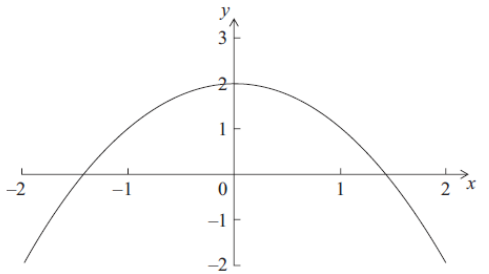
\includegraphics[scale=0.4]{figure_x24}\par
  \end{center} % or flushleft or flushright
  \begin{enumerate}[label=(\alph*)]
    \item Sur la figure ci-dessus, esquissez la représentation graphique de $g$.\hspace*{\fill} [3]
    \item Resolvez $f(x) = g(x)$.\hspace*{\fill} [2]
    \item Donnez lensemble des valeurs de x telles que $f(x) > g(x)$.\hspace*{\fill} [2]
  \end{enumerate}
\end{question}
